\documentclass[14pt, a4paper]{report}
\usepackage{mathtext}
\usepackage[T2A]{fontenc}
\usepackage[utf8]{inputenc}
\usepackage[russian]{babel}
\usepackage{multirow}
\usepackage{slashbox}
\usepackage{makecell}
\usepackage{graphicx}
\usepackage{physics}
\usepackage{amstext}
\usepackage{caption}
\usepackage{subcaption}
\usepackage{cmap}
\usepackage{float}

\renewcommand{\thesection}{\arabic{section}.}
\renewcommand{\thesubsection}{\arabic{section}.\arabic{subsection}.}

\title{\textbf{Отчет о выполнении лабораторной работы 3.2.5 "Свободные и вынужденные колебания в электрическом контуре"}}
\author{Алпатова Александра и Калашников Михаил, Б03-205}
\date{}

\begin{document}
\maketitle

\textbf{Цель работы:}
исследование свободных и вынужденных колебаний в колебательном контуре.
\newline

\textbf{В работе используются:}
\begin{itemize}
\item осциллограф AKTAKOM ADS-6142H;
\item генератор сигналов специальной формы АКИП-3409/4;
\item магазин сопротивления МСР-60;
\item магазин емкости Р5025;
\item магазин индуктивности Р567 типа МИСП;
\item соединительная коробка с шунтирующей емкостью;
\item соединительные одножильные и коаксиальные провода.
\end{itemize}

\section{Теоретические сведения}

\section{Экспериментальная установка}


\section{Проведение эксперимента}

\subsection{Подготовка приборов к работе}

\begin{enumerate}

\setcounter{enumi}{0}

\item Подключим генератор специальных сигналов к входу 1(X) осциллографа.

\item Установим на генераторе сигналов последовательность импульсов.

\item Получим на осциллографе статичное изображение сигнала.

\item Соберем схему как на рис. 1.

\end{enumerate}

\subsection{Измерение периодов свободных колебаний}

\begin{enumerate}

\setcounter{enumi}{0}

\item Выставим на магазине сопротивлений нулевое сопротивление, а на магазине индуктивностй $L=100\ мГн$, на магазине емкостей нулевую емкость. В таком случае в контур реализуются свободные колебания из-за собственной емкости $C_0$ контура и активного сопротивления катушки $R_L$.

\item Получим на экране осциллографа статичное изображение сигнала.

\item Измерим с помощью курсоров осциллографа период затухающих колебаний.

\item По периоду колебний определим нулевую емкость $C_0$ колебательного контура.

\item Изменяя емкость от $0\ мкФ$ до $0.009\  мкФ$ проведем измерения периодов.

\item Рассчитаем экспериментальное значение периодов по результатам измерений.

\end{enumerate}

\subsection{Критическое сопротивление и декремент затухания}

\begin{enumerate}

\setcounter{enumi}{0}

\item Приняв $L=100\ мГн$, рассчитаем емкость $C^*$, при которой собственная частота колебаний $\nu_0$ составляет $6.5\ кГц$: $C=\frac{1}{(2\pi\nu_0)^2L}=0.006\ мкФ$. Рассчитам критическое сопротивление контура: $R_{cr}=2\sqrt{L/C^*}=8.16\ кОм$.

\item Установим на магазине критическую емкость.

\item Установим сопротивление $R=0.05R_{cr}$. Получим на экране картину затухающих колебаний. Проведем измерения амплитуд соседних колебаний.

\item Повторим измерения для еще 5 значений сопротивлений в диапазоне $(0.05-0.25)R_{cr}$.

\item Занесем результаты измерений в таблицу. Погрешность измерения напряжения составила $\sigma_U=4\ мВ$.

\item Рассчитаем значения логарифмического декремента затухания по формуле:
\[\Theta=\ln{\frac{U_1}{U_2}}\]
Далее можно рассчиать добротность контура как $Q=\pi/\Theta$.

\begin{table}[H]
\centering
\makebox[\textwidth][c] {
\begin{tabular}{| c | c | c | c | c | c | c |}
\hline
$R/R_{cr}$ & 0.05 & 0.09 & 0.14 & 0.18 & 0.23 & 0.25 \\
\hline
$U_1,\ мВ$ & $684\pm4$ & $648\pm4$ & $604\pm4$ & $576\pm4$ & $536\pm4$ & $528\pm4$ \\
$U_2,\ мВ$ & $468\pm4$ & $336\pm4$ & $220\pm4$ & $160\pm4$ & $104\pm4$ & $92\pm4$   \\
$\Theta$ & $0.379\pm0.010$ & $0.657\pm0.013$ & $1.010\pm0.019$ & $1.28\pm0.03$ & $1.64\pm0.04$ & $1.75\pm0.04$ \\
$Q$ & $8.3\pm0.2$ & $4.8\pm0.1$ & $3.11\pm0.06$ & $2.45\pm0.05$ & $1.92\pm0.05$ & $1.80\pm0.05$ \\
\hline
\end{tabular}
}
\caption{Результаты измерения амплитуд соседних колебаний}
\end{table}

\item Основываясь на результатах измерения активного сопротивления, проведем линейную экстраполяцию и получим зависимость $R_L(\nu)$. Рассчитаем значения $R_{\Sigma}=R+R_L(\nu_0)$ и построим график зависимости $1/\Theta^2=f(1/R_{\Sigma}^2)$.

\begin{figure}[H]
\centering
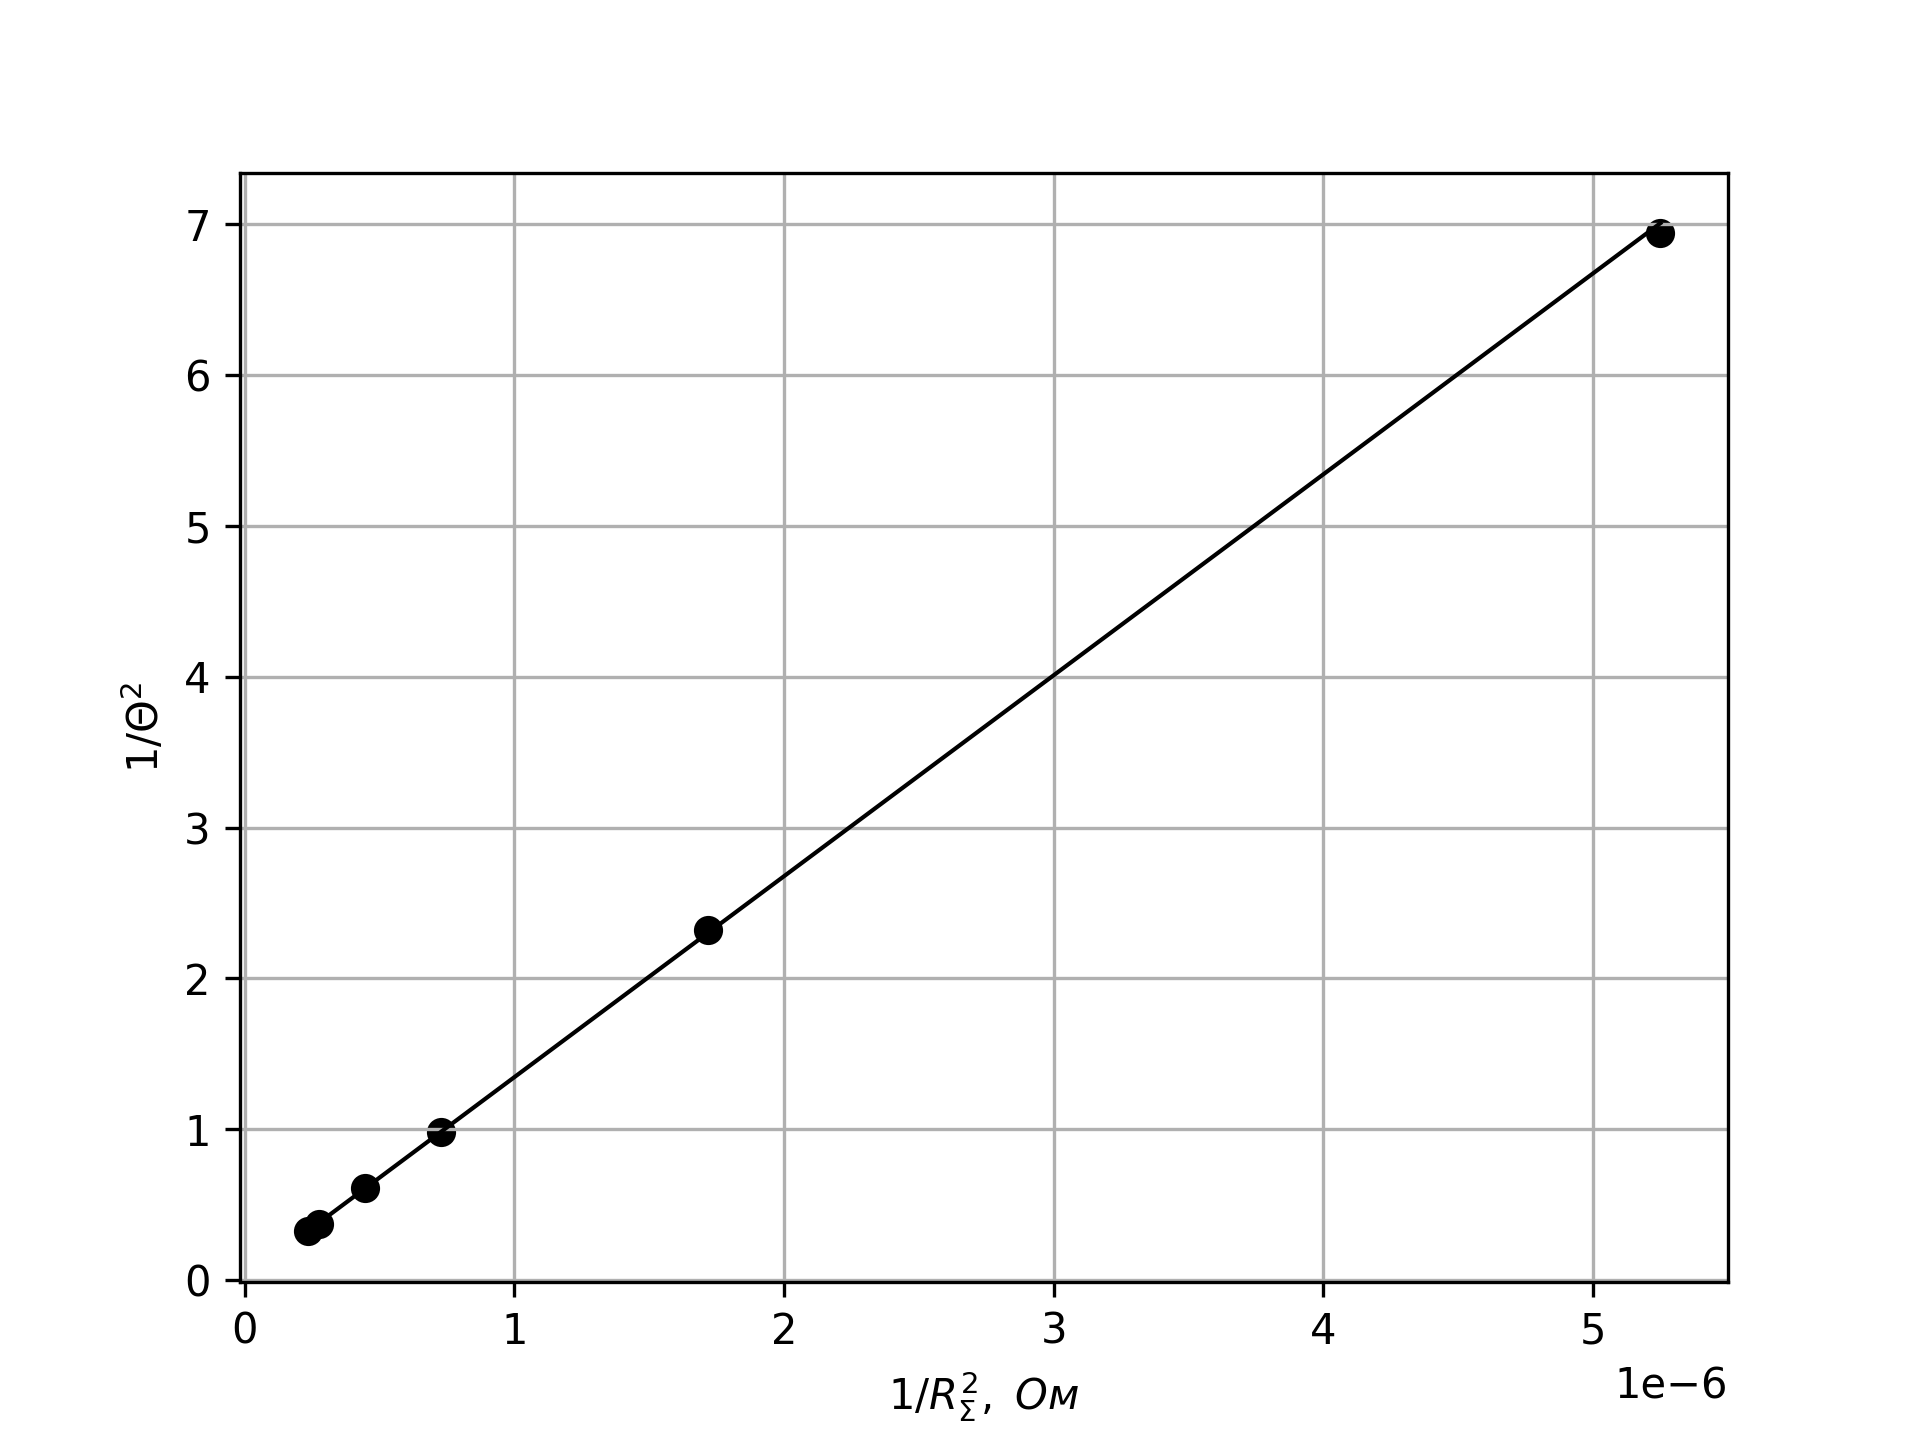
\includegraphics[scale=0.6]{images/325_1.png}
\caption{График зависимости $1/\Theta^2=f(1/R_{\Sigma}^2)$}
\end{figure}

По наклону графика $k$ определим критическое сопротивление как $R_{cr, exp}=2\pi\sqrt{k}=7.25\pm0.03\ кОм$.

\end{enumerate}

\subsection{Свободные колебания на фазовой плоскости}

\begin{enumerate}

\setcounter{enumi}{0}

\item Выставим на магазине сопротивлений сопротивление $R=0.05R_{cr}$. На канал 2(Y) осциллографа подадим падение напряжения на резисторе.

\item Переведем осциллограф в двухканальный режим работы.

\item Выставим на генераторе частоту $500\ Гц$.

\item Пронаблюдаем изменение спирали при увеличении сопротивления от $0.05R_{cr}$ до $0.25R_{cr}$. С помощью программы Paint измерим координаты пересечения соседних пересечений витков спирали с положительным направлением оси OX. Погрешность таких измерий имеет примерно тот же порядок, что и погрешность предыдущих. Для простоты приравняем их.

\item Логарифмический декремент затухания и добротность могут быть найдены по формулам из прошлого раздела.

\begin{table}[H]
\centering
\makebox[\textwidth][c] {
\begin{tabular}{| c | c | c | c | c | c | c |}
\hline
$R/R_{cr}$ & 0.05 & 0.09 & 0.14 & 0.18 & 0.23 & 0.25 \\
\hline
$U_1,\ мВ$ & $562\pm4$ & $449\pm4$ & $362\pm4$ & $298\pm4$ & $233\pm4$ & $208\pm4$ \\
$U_2,\ мВ$ & $377\pm4$ & $230\pm4$ & $131\pm4$ & $77\pm4$ & $43\pm4$ & $32\pm4$ \\
$\Theta$ & $0.399\pm0.013$ & $0.67\pm0.02$ & $1.02\pm0.03$ & $1.35\pm0.05$ & $1.70\pm0.10$ & $1.87\pm0.13$ \\
$Q$ & $7.8\pm0.3$ & $4.69\pm0.14$ & $3.08\pm0.10$ & $2.33\pm0.09$ & $1.85\pm0.10$ & $1.68\pm0.11$ \\
\hline
\end{tabular}
}
\caption{Результаты измерения координат пересечения соседних витков спирали}
\end{table}

\end{enumerate}

\subsection{Исследование резонансных кривых}

\begin{enumerate}

\setcounter{enumi}{0}

\item Переведем осциллограф в одноканальный режим работы.

\item Переведем генератор сигналов в режим подачи синусоидального сигнала.

\item Выставим емкость $C^*$ и сопротивление $0.05R_{cr}$

\item С помощью тройника подадим на канал 2(Y) осциллографа сигнал напрямую с генератора.

\item Убедимся что на экране наблюдается устойчивый синусоидальный сигнал.

\item Изменяя частоту вблизи резонансной, обнаружим, что та максимальна при $\nu=6\ кГц$. Снимем АЧХ и ФЧХ с осциллографа (($U_1$ и $\tau_1$)).

\item Установим сопротивление $0.25R_{cr}$ и повторим измерения ($U_2$ и $\tau_2$). Погрешность измерений составила $\sigma_{U_1}=0.04\ В$, $\sigma_{U_2}=0.02\ В$, $\sigma_{\tau_1}=1\ мкс$, $\sigma_{\tau_2}=0.2\ мкс$ 

\begin{table}[H]
\centering
\makebox[\textwidth][c] {
\begin{tabular}{| c | c | c | c | c | c | c | c |}
\hline
$\nu,\ кГц$ & 5.0 & 5.1 & 5.2 & 5.3 & 5.4 & 5.5 & 5.6 \\
\hline
$U_1,\ В$ & 2.24 & 2.54 & 2.90 & 3.30 & 3.84 & 4.46 & 5.40 \\
$\tau_1,\ мкс$ & 84 & 83 & 78 & 74 & 72 & 68 & 63 \\
$U_2,\ мВ$ & 1.54 & 1.61 & 1.67 & 1.74 & 1.83 & 1.89 & 1.95 \\
$\tau_2,\ мкс$ & 49.2 & 48.0 & 44.4 & 41.6 & 40.4 & 38.4 & 34.0 \\
\hline
$\nu,\ кГц$ & 5.7 & 5.8 & 5.9 & 6.0 & 6.1 & 6.2 & 6.3 \\
\hline
$U_1,\ В$ & 6.28 & 7.24 & 7.96 & 8.24 & 8.04 & 7.40 & 6.68 \\
$\tau_1,\ мкс$ & 58 & 51 & 43 & 37 & 31 & 23 & 18 \\
$U_2,\ мВ$ & 1.99 & 2.04 & 2.08 & 2.11 & 2.13 & 2.15 & 2.15 \\
$\tau_2,\ мкс$ & 31.6 & 32.8 & 30.4 & 27.2 & 26.0 & 22.8 & 22.4 \\
\hline
$\nu,\ кГц$ & 6.4 & 6.5 & 6.6 & 6.7 & 6.8 & 6.9 & 7.0 \\
\hline
$U_1,\ В$ & 6.00 & 5.40 & 4.92 & 4.32 & 4.02 & 3.74 & 3.48 \\
$\tau_1,\ мкс$ & 14.0 & 13.0 & 11.0 & 10.4 & 7.6 & 6.4 & 7.2 \\
$U_2,\ мВ$ & 2.14 & 2.14 & 2.14 & 2.13 & 2.12 & 2.10 & 2.08 \\
$\tau_2,\ мкс$ & 20.4 & 20.4 & 18.8 & 17.8 & 16.0 & 15.2 & 14.2 \\
\hline
\end{tabular}
}
\caption{Результаты измерения АЧХ и ФЧХ}
\end{table}

\begin{figure}[H]
\centering
\makebox[\textwidth][c] {
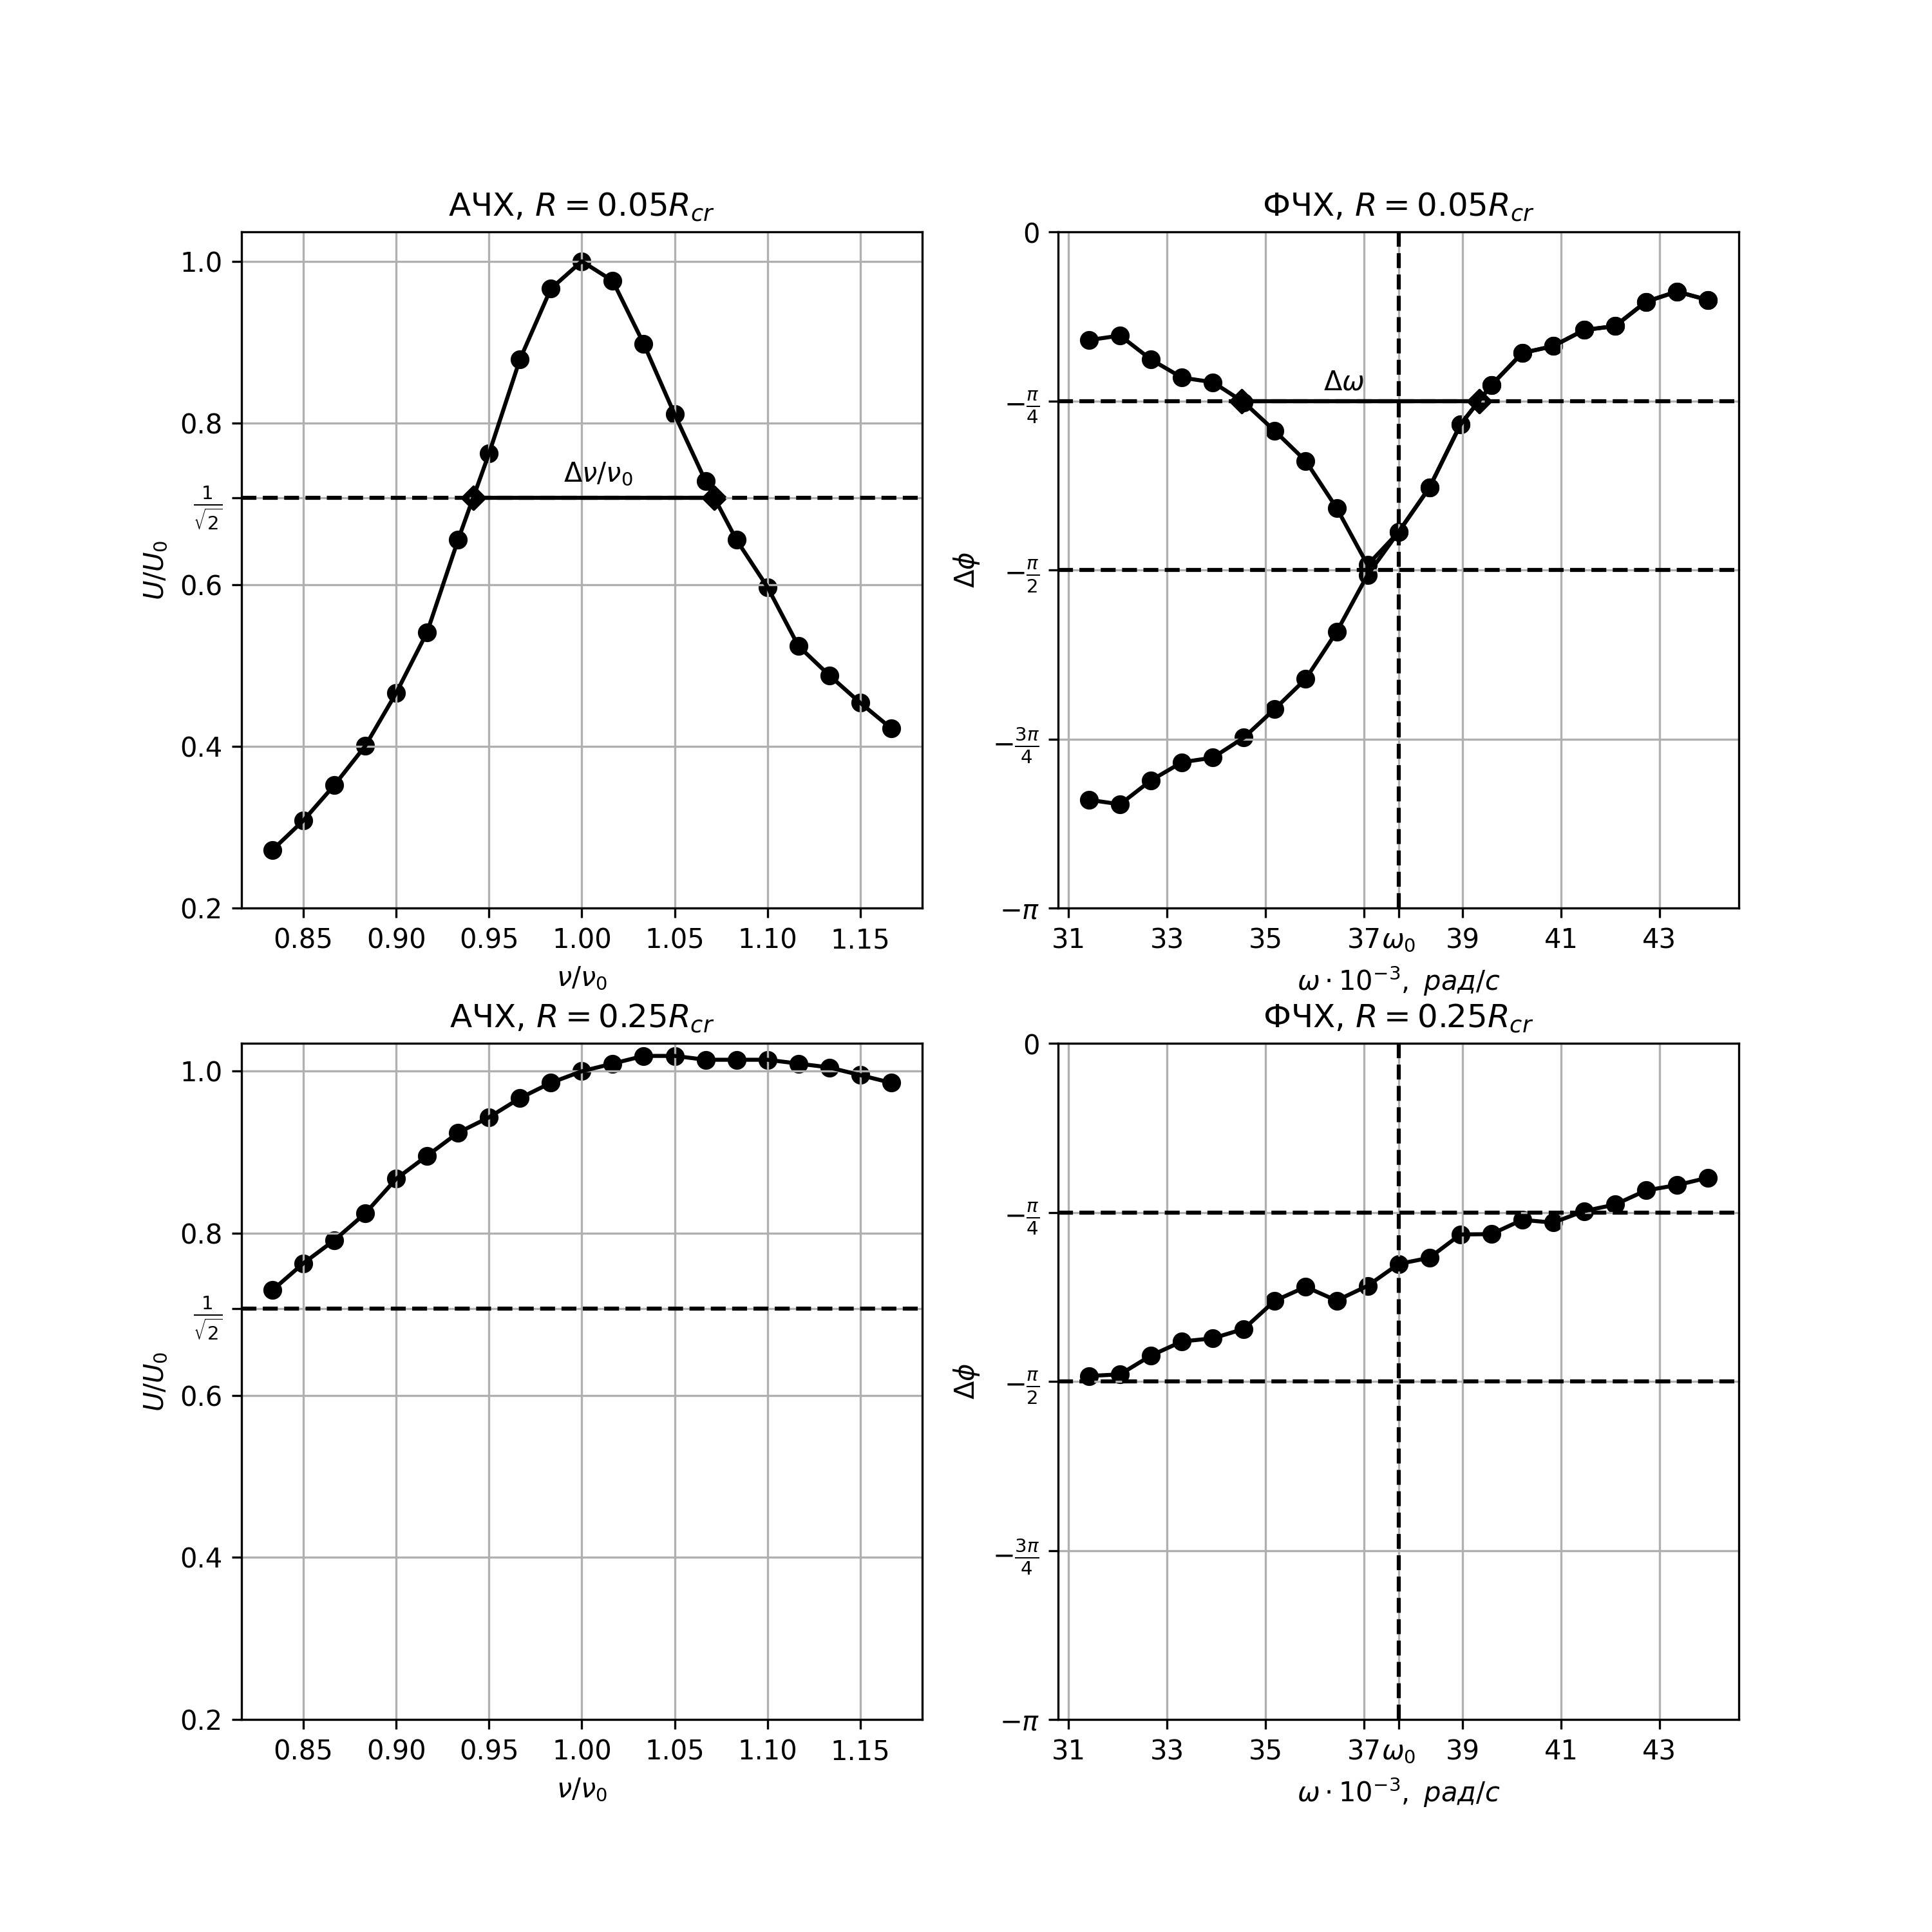
\includegraphics[scale=0.6]{images/325_2.png}
}
\caption{АЧХ и ФЧХ для двух различных сопротивлений}
\end{figure}

\item По графикам определим добротность контура. При работе со вторым сопротивлением было проведено измерение слишком маленького количества точек. Это препятствует графическому измерению добротности. Для первого сопротивления: $\Delta\nu=780\pm13\ Гц$, $\Delta\omega=4.82\pm0.08\ \frac{рад}{с}$. Рассчитаем добротности: $Q_{АЧХ}=\frac{1}{\nu/\nu_0}=7.68\pm0.13$, $Q_{ФЧХ}=\frac{1}{\omega/\omega_0}=7.82\pm0.13$.

\end{enumerate}

\subsection{Процессы установления и затухания}

\begin{enumerate}

\setcounter{enumi}{0}

\item Вернем на магазин сопротивлений $0.05R_{cr}$.

\item Установим на генераторе резонансную частоту.

\item Включим на генераторе режим "Burst".

\item Установим режим повторения сигнала $20\ мс$, а количество периодов -- 15.

\item Получим на экране осциллографа картинку установления и затухания одного цуга.

\item Измерим амплитуды двух колебаний, разделенных одним периодом, и амплитуду установившихся колебаний.

\item Повторим измерения для затухающего участка.

\item Повторим измерения для сопротивления $0.25R_{cr}$. Погрешность измерения амплитуд для первого сопротивления составляет $\sigma_{U_1}=0.01\ В$, а во втором -- $\sigma_{U_2}=0.004\ В$.

\begin{table}[H]
\centering
\makebox[\textwidth][c] {
\begin{tabular}{| c | c | c | c | c | c |}
\hline
& $U_0,\ мВ$ & $U_1,\ мВ$ & $U_2,\ мВ$ & $U_3,\ мВ$ & $U_4,\ мВ$ \\
\hline
$0.05R_{cr}$ & $1620\pm10$ & $560\pm10$ & $1150\pm10$ & $1110\pm10$ & $520\pm10$ \\
$0.25R_{cr}$ & $444\pm4$ & $156\pm4$ & $380\pm4$ & $372\pm4$ & $68\pm4$ \\
\hline
\end{tabular}
}
\caption{Результаты измерения амплитуды затухающих колебаний}
\end{table}

Тогда логарифмические декременты при установлении и затухании можно найти по формулам:
\[\Theta_{нар}=\frac{1}{2}\ln{\frac{U_0-U_1}{U_0-U_2}}\]
\[\Theta_{зат}=\frac{1}{2}\ln{\frac{U_3}{U_4}}\]

\begin{table}[H]
\centering
\makebox[\textwidth][c] {
\begin{tabular}{| c | c | c | c |}
\hline
& $\Theta_{нар}$ & $\Theta_{зат}$ \\
\hline
$0.05R_{cr}$ & $7.7\pm0.2$ & $8.3\pm0.3$ \\
\hline
$0.25R_{cr}$ & $4.2\pm0.2$ & $3.70\pm0.17$ \\
\hline
\end{tabular}
}
\caption{Вычисление добротности по амплитудам затухающих колебаний}
\end{table}


\item Сместим частоту генератора с резонансной и получим картину биений. Они появляются в результате того, что решением уравнения вынужденный колебаний является линейная сумма гармонических функций, которая сводится к произведение двух гармонических сигналов.

\item Проведем измерение активного сопротивления $R_L$ и индуктивности $L$ магазина индуктивностей с помощью измериятся LCR на разных частотах.

\begin{table}[H]
\centering
\makebox[\textwidth][c] {
\begin{tabular}{| c | c | c | c |}
\hline
$\nu,\ Гц$ & 50 & 500 & 1500 \\
\hline
$R_L,\ Ом$ & 21.631 & 21.874 & 23.080 \\
\hline
$L,\ мГн$ & 99.991 & 99.964 & 99.998 \\
\hline
\end{tabular}
}
\caption{Результаты измерения активного сопротивления и индуктивности магазина индуктивностей}
\end{table}

\end{enumerate}

\section{Вывод}

\begin{table}[H]
\centering
\makebox[\textwidth][c] {
\begin{tabular}{| c | c | c | c | c | c | c | c |}
\hline
& \multicolumn{3}{ c |}{Свободные колебания} & \multicolumn{4}{ c |}{Вынужденные колебания} \\
\cline{2-8}
& $f(L, C, R)$ & $f(\Theta)$ & Спираль & АЧХ & ФЧХ & Нарастание & Затухание \\
\hline
$R=0.05R_{cr}$ & 10 & $8.3\pm0.2$ & $7.8\pm0.3$ & $7.68\pm0.13$ & $7.82\pm0.13$ & $7.7\pm0.2$ & $8.3\pm0.3$ \\
\hline
$R=0.25R_{cr}$ & 2 & $1.80\pm0.05$ & $1.68\pm0.11$ & - & - & $4.2\pm0.2$ & $3.70\pm0.17$ \\
\hline
\end{tabular}
}
\caption{Итоговая таблица}
\end{table}


\end{document}